\documentclass[preprint,11pt]{elsarticle}
\usepackage[margin=2.5cm]{geometry}
\usepackage{algpseudocode}
\usepackage{amsmath}
\usepackage{amssymb}
\usepackage{amsthm}
\usepackage{amsfonts}
\usepackage{graphicx}
\usepackage{hyperref}
\usepackage{titlesec}
\usepackage{multicol}
\usepackage{float}
\usepackage{array}
\usepackage[ruled,vlined]{algorithm2e}
\usepackage{microtype}
\usepackage{natbib}


\theoremstyle{definition}
\newtheorem{theorem}{Theorem}
\newtheorem*{manualtheorem}{Theorem}
\newtheorem{lemma}[theorem]{Lemma}  
\newtheorem{proposition}[theorem]{Proposition}


\renewcommand\thesection{\Roman{section}}
\titleformat{\section}[block]{\filcenter\bfseries}{\thesection.}{1em}{}
\title{\centering \textbf{Testing Graph Properties with the Container Method}}
\author{
    \begin{tabular}{>{\centering\arraybackslash}p{0.45\textwidth} >{\centering\arraybackslash}p{0.45\textwidth}}
        Eric Blais & Cameron Seth \\
        David R. Cheriton School of Computer Science & David R. Cheriton School of Computer Science \\
        University of Waterloo & University of Waterloo \\
        \emph{Waterloo, Canada} & \emph{Waterloo, Canada} \\
        \emph{\texttt{eric.blais@uwaterloo.ca}} & \emph{\texttt{cjmpseth@uwaterloo.ca}} \\
    \end{tabular}
}

\begin{document}
\maketitle
\begin{multicols}{2}
\textbf{\textit{Abstract-}
We establish nearly optimal sample complexity bounds for testing the $\rho$-clique property in the dense graph model. Specifically, we show that it is possible to distinguish graphs on $n$ vertices that have a $\rho n$-clique from graphs for which at least $\epsilon n^2$ edges must be added to form a $\rho n$-clique by sampling and inspecting a random subgraph on only $\tilde{O}(\rho^3/\epsilon^2)$ vertices.\\ We also establish new sample complexity bounds for $\epsilon$-testing $k$-colorability. In this case, we show that a sampled subgraph on $\tilde{O}(k/\epsilon)$ vertices suffices to distinguish $k$-colorable graphs from those for which any $k$-coloring of the vertices causes at least $\epsilon n^2$ edges to be monochromatic.\\The new bounds for testing the $\rho$-clique and $k$-colorability properties are both obtained via new extensions of the graph container method. This method has been an effective tool for tackling various problems in graph theory and combinatorics. Our results demonstrate that it is also a powerful tool for the analysis of property testing algorithms.
}
\section{Introduction}
The paper discusses the problem of testing if a graph contains a large clique or is k-colorable by examining only a small fraction of the graph.It introduces the concept of a canonical tester,which samples a subset of vertices and examines the induced subgraph to determine if the graph has a certain property.The sample complexity for testing the $\rho$-CLIQUE property is shown to be ($\tilde{O}(\rho^3/\epsilon^2$)), which is nearly optimal . This result has been significant implications , especially in the small clique regime , where the sample complexity is sublinear in ($n$) for certain values of {$\rho$} and {$\epsilon$}.
\subsection*{\textit{\textbf{A.Testing Cliques}}}
    The problem of testing the \textbf{$\rho$-CLIQUE property} in graphs, which focuses on determining whether the graph contains a large clique on $\rho n$ vertices.The problem can be analyzed in two regime - Large Clique Regime where $\rho$ is a constant,meaning the size of the clique is a fixed proportion of the graph's vertices.Small Clique Regime where $\rho$ is a function of the graph size ($n$),typically when $\rho$ is small relative to $n$.
    \\Here the sample complexity refers to how many vertices need to be sampled from a graph to test if it has a $\rho n$-clique or not.Goldreich, Goldwasser, and Ron \cite{GGR98} were the first to consider the quetion and showed that $S_{\rho-{\text{CLIQUE}}}(n,\epsilon) = \tilde{O}(\rho/\epsilon^4)$.In the large clique regime,it shows that $\epsilon$-testing $\rho$-clique property is sublinear in $n$ for all $\rho=\omega(n^{-1/7}$ when $\epsilon=\Omega(\rho^2)$ -- i.e.,when the tester must distinguish graphs with $\rho n$-cliques from those whose $\rho n$-subgraphs all have constant density bounded by 1.Then there is a improved upperbound of $S_{\rho-\text{CLIQUE}}(n,\epsilon)=\tilde{O}(\rho^4/\epsilon^3)$ provided by Feige, Langberg, and Schechtman \cite{FLS04}.
    
    Additionally,they established a lower bound of $S_{\rho-\text{CLIQUE}}(n,\epsilon)=\tilde{\Omega}(\rho^3/\epsilon^2)$, meaning any testing algorithm will require at least this many samples to work efficiently.
    
   The authors present a new upper bound on the sample complexity of testing the $\rho$-CLIQUE property that nearly matches the previously established lower bound, up to polylogarithmic factors. This implies that their result is close to the optimal solution for this problem.The results are significant in property testing, where the goal is to determine graph properties by examining a small sample, rather than the entire graph.
 \begin{figure}[H]
    \centering
    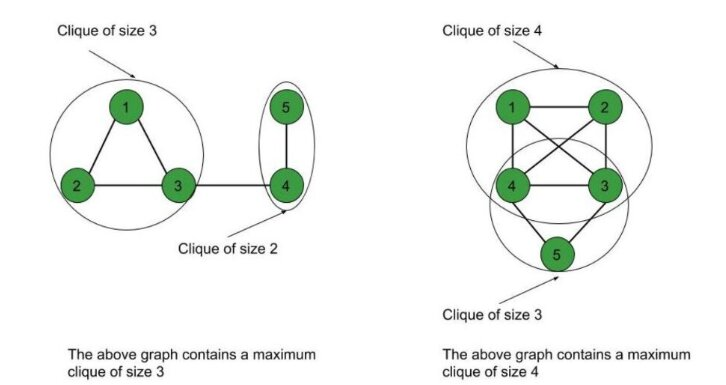
\includegraphics[width=\columnwidth]{images/graphClique.jpg} 
    \caption{Graph Clique}\cite{GFG2024a}
    \label{fig:Fig 1}
\end{figure}
\begin{theorem}\textit{Sample Complexity of the $\rho$-CLIQUE Property is $S_{\rho-CLIQUE}(n,\epsilon)=\tilde{O}(\frac{\rho^3}{\epsilon^2})^2$}.
This theorem establishes the sample complexity for testing the $\rho$-CLIQUE property in a graph. Specifically, it shows that Sample Complexity $S_{\rho-\text{CLIQUE}}(n,\epsilon)=\tilde{\Omega}(\rho^3/\epsilon^2)$. This result implies that you can test whether a graph  contains a large clique or is far from having a large clique by inspecting a relatively small number of vertices. The bound is near-optimal, matching known lower bounds up to polylogarithmic factors.
\end{theorem}
\begin{manualtheorem}[1'][Alternative Formulation]
 For any $n , k=k(n) < n$, and $\delta:=\delta(n) > 0$ a randomized algorithm can distinguish between Graphs containing $k$-cliques and Graphs where every $k$-subgraph contains at most $(1-\delta)k^2$ edges.Here we only need to inspect a random subset of $|S|=O(n/(\delta^2k){ln^3(n/(\delta^2k))}$ vertices.This formulation shows that if $k$ grows faster than $\ln^3{n}$, you can distinguish between these two types of graphs by examining a sublinear portion of the graph.
 The result generalizes the previous findings Previous bounds showed sublinear sample complexity for specific values of $k$ by Feige, Langberg, and Schechtman \cite{FLS04}. The results build on these earlier works related to Planted $k$-Clique Detection, showing similar sample complexity bounds for the Densest $k$-Subgraph problem given by Racz and Schiffer \cite{RS19} and Huleihel, Mazumdar, and Pal \cite{HMP21}.\\
For algorithms that can query any vertex pair (as opposed to sampling vertices), Theorem 1’ also provides a nearly optimal upper bound on the number of queries needed $O(n^2/(\delta^4k^2)ln^6(n/(\delta^2k)))$.
\end{manualtheorem}
\subsection*{\textit{\textbf{B.Testing Colorability}}}
The discussion focuses on the problem of testing the $k$-COLORABLE property for graphs, where a graph is $k$-colorable if its vertices can be colored with $k$ colors such that no two adjacent vertices share the same color.For $k=2$, which corresponds to testing bipartiteness , nearly optimal bounds $S_{2-\text{COLORABLE}}(n,\epsilon)=\tilde{\Theta}(1/\epsilon)$ \cite{GGR98},\cite{AK02} are known.For $k\geq 3$ ,there is low chromatic number regime.When $k$ is constant ,Rodl and Duke \cite{RD85} demonstrated that $S_{k-\text{COLORABLE}}(n,\epsilon)$
is constant when both $k$ and $\epsilon$ is constants.However ,this result is limited to very large values of $k$ when $\epsilon$ is small. For $k$ as a function of $n$ , Goldreich, Goldwasser, and Ron (1998) \cite{GGR98} provided that $S_{k-\text{COLORABLE}}(n,\epsilon)=\tilde{O}(k^2/\epsilon^3)$ for all $k\geq 3$.This shows $k$-colorability is testable with sublinear complexity for small $\epsilon$ when $k=o(n^{1/5})$ . Alon and Krivelevich (2002) \cite{AK02} improved the bound to $S_{k-\text{COLORABLE}}(n,\epsilon)=\tilde{O}(k/\epsilon^3)$, showing the $k$-colorability is testable with sublinear complexity for all $k=o(n^{1/3})$ Sohler (2012) \cite{Soh12} provided that
$S_{k-\text{COLORABLE}}(n,\epsilon)=\tilde{O}(k^6/\epsilon)$ for low chromatic numbers, where the bound is optimal when $k$ is constant. In the polychromatic regime, the bounds of Alon and Krivelevich are stronger for large $k$ and small $\epsilon$.
\begin{theorem}\textit{The $k$-COLORABLE property has sample complexity $S_{k-COLORABLE}(n,\epsilon)=\tilde{O}(k/\epsilon)$.}
This theorem states  that the sample complexity for testing  $k$-COLORABLE property is $S_{k-\text{COLORABLE}}(n,\epsilon)=\tilde{O}(k/\epsilon)$. This result unifies and improves upon previous results, demonstrating that sublinear sample complexity is sufficient to distinguish $k$-colorable graphs from graphs where any  $k$-coloring results in at least $\delta/k$ monochromatic edges for  $k=o(\sqrt{n})$ and constant $\delta>0$.The lower bound for testing 
$k$-colorability in the polychromatic regime is  $\omega(1/\epsilon) $[AK02]. This indicates a quadratic gap between the upper bound provided by Theorem 2 and the best-known lower bound for large $k$.
\end{theorem}
\begin{figure}[H]
    \centering
    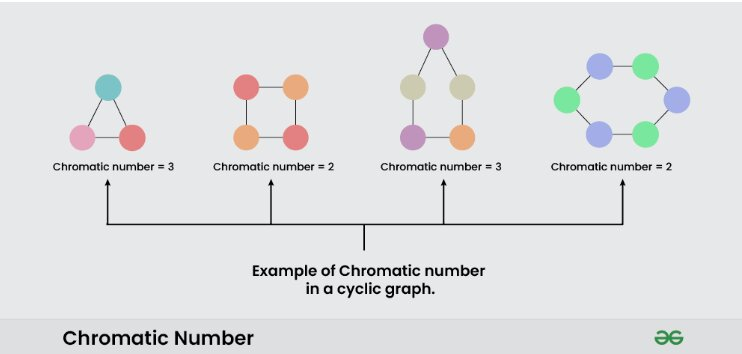
\includegraphics[width=\columnwidth]{images/graphColor.jpg} 
    \caption{Graph Color}\cite{GFG2024b}
    \label{fig:Fig 2}
\end{figure}
\subsection*{\textit{\textbf{C.The Graph Container Method}}}
The text describes the use of the graph container method to address challenges in property testing, specifically for testing $\rho$-cliques and $k$-colorability. The method involves finding a smaller collection of "containers" for independent sets within a graph. Each independent set is a subset of at least one container, and each container is small and sparse. The goal is to simplify the analysis of property testing by focusing on these containers.
\subsection*{Testing $\rho$-independence}
The method is applied to test $\rho$-independent sets, which is equivalent to testing $\rho$-cliques in the complement graph.
Key technical lemmas provide tight bounds on the size of containers based on the size of their fingerprints.
The probability that a sample contains a large independent set is bounded using these containers and their fingerprints.
\subsection*{Testing $k$-colorability}
Similar to $\rho$-independence, the method is applied to test $k$-colorability, but a different argument is used.
The text hints at the application of the hypergraph container method for partition properties of hypergraphs, which might offer new insights for property testing in other domains.\\
It is discussed how the query complexity of adaptive testers (which can query any edge) compares to the canonical tester (which samples vertices and queries edges within the induced subgraph).
For large cliques, Theorem 1 indicates that the number of edge queries for the canonical tester is close to the query complexity of the best adaptive tester when 
$\epsilon=\Omega(\rho^2)$
For k-colorability, the open question is whether adaptivity can improve query complexity, particularly for $\epsilon$ smaller than $\epsilon=\Omega(\rho^2)$.\\
Theorem 1' provides a bound on the sample complexity of the Densest $k$-Subgraph problem, which also implies results on time complexity.For distinguishing graphs with k-cliques from those with k-subgraphs of density at most $(1-\delta)$ ,sampling $s=O(n^{\delta^2k}ln^3(n^{\delta^2k}))$ vertices suffices.Checking whether the induced subgraph contains a clique of size \\$O(\delta^{-2}ln^3(n^{\delta^2k})$ results in quasipolynomial time complexity $n^{O(ln^3n)}$.
\subsection*{\textit{\textbf{D.Discussion}}}
The discussion highlights several open problems related to the graph container method and its application to property testing:
\subsection*{ 1.Property Testing with the Container Method:}
The method is effective for testing cliques and colorability and may extend to other $0-1$graph partition properties \cite{NR18}. Future work could explore its application to more general graph properties and hypergraph partition properties.
\subsection*{2.Query Complexity:}The relationship between adaptive testers querying any edge and canonical testers sampling vertices is still open. Theorem 1 suggests that the query complexity for testing large cliques is close to the best adaptive testing algorithm when 
$\epsilon=\Omega(\rho^2)$. Questions remain about whether adaptivity can reduce queries further, especially for testing bipartiteness with 
$O(n^2)$queries \cite{BL10}.
\subsection*{3.Time Complexity:}
Theorem 1' provides bounds for the Densest $k$-Subgraph problem, showing that distinguishing graphs with $k$-cliques from those with lower density subgraphs can be done with sampling 
$s=O({n^{\delta^2k}ln^3(n^{\delta^2k})}/{\delta^2k})$ vertices and checking for cliques of size $O({\delta^{-2}ln^3(n^{\delta^2k}}/n)$ , resulting in quasipolynomial time complexity 
$n^{O(ln^3n)}$. Improvements in time complexity for property testing could be achieved using the container method.
\section{The Container Method}
The container method involves a process to study independent sets in graphs through a specific greedy algorithm, which is a variant of the approach initially proposed by Kleitman and Winston \cite{KW82}. This method uses fingerprints and containers to manage and analyze independent sets.
\begin{algorithm}[H]
\LinesNumbered
\KwIn{A graph $G = (V, E)$ and an independent set $I \subseteq V$}
Initialize $F_0 \gets \emptyset$ and $C_0 \gets V$\;
\For{$t = 1, 2, \dots, |I|$} 
    {$v_t \gets$ the vertex in $I \setminus F_{t-1}$ with the largest degree in $G[C_{t-1}]$\;
    \tcp{Add $v_t$ to the fingerprint}
    
    $F_t \gets F_{t-1} \cup \{v_t\}$\;   
    \tcp{Remove all the neighbors of $v_t$ from the container}  
    
    $C_t \gets C_{t-1} \setminus \{w \in C_{t-1} : (v, w) \in E \}$\;
    \tcp{And remove all vertices with higher degree than $v_t$ in $G[C_{t-1}]$}

    $C_t\gets C_t\setminus \{w \in C_{t-1}:\text{deg}_{G[C_{t-1}]}(w) > \text{deg}_{G[C_{t-1}]}(v_{t})\}$\;
    }
\KwRet{$F_1,\dots,F_{|I|}$ and $C_1,\dots,C_{|I|}$}\;
\caption{FINGERPRINT \& CONTAINER GENERATOR}
\end{algorithm}
\subsection*{\textbf{A.Basic Properties of Container}}
\subsubsection*{1.Containment Relation:}
\begin{equation}
  \resizebox{\columnwidth}{!}{$
  F_1 \subseteq F_2 \subseteq F_3 \subseteq F_4 \subseteq \cdots \subseteq F_{|I|} = I \subseteq C_{|I|} \subseteq C_{|I|-1} \subseteq \cdots \subseteq C_2 \subseteq C_1  
  $}
  \tag{1}
\end{equation}
\\Each fingerprint is a subset of the independent set $I$, and each container is a superset.
\subsubsection*{2.Container Consistency:}There is a proposition about this topic.
\begin{proposition}
For any $t$,
\begin{equation*}
C_T(F_t(I))=C_t(I)
\end{equation*}.This means that the container for $F_t(I)$ is the same as the container for $I$ at the same stage.
\end{proposition}
\subsubsection*{3.Degree Bound:}There ia also a proposition about the maximum desgree bound about the graph container method.
\begin{proposition}
The maximum degree in $G[C_t]$ is bounded  by \\$\Delta(G[C_t])\leq (n/t)$.This follows from the fact that vertices are excluded based on their degrees, ensuring that no vertex in $C_t$ has a degree exceeding $n/t$ in the included subgraph.This method and its properties are valuable in understanding the structure of independent sets and can be applied to various problems in graph theory and combinatorics.
\end{proposition}
\subsection*{\textbf{B. Graph Container Lemmas}} 
In the case of testing the $\rho$-CLIQUE property, we first change our focus so that we instead look at graphs that are $\epsilon$-far from having the $\rho$-INDEPENDENT SET property. We show that for each such graph $G$, every independent set in $G$ is a subset of a container
of size strictly less than $\rho n$. In fact, our result shows more:
there is a container for $I$ of size $(\rho-\alpha)n$ where $\alpha$ is at least as large as $\epsilon/\rho$ times the length of the corresponding fingerprint(up to log factors).
\begin{lemma}[\textit{Graph Container Lemma I}]
For a graph $G=(V,E)$ that is $\epsilon$-far from the $\rho$-INDEPSET property, every independent set $I$ is a subset of a container $C_t$,where size of the  container bounded as :
\begin{equation}
|C_t|\leq(\rho-t.\frac{\epsilon}{{8\rho\ln(2\rho)}})n
\tag{2}
\end{equation}
Additionally, the induced subgraph $G[C_t]$ contains at most $\epsilon n^2$ edges.
\end{lemma}
\begin{lemma}[\textit{Graph Container Lemma II}]
For graphs that are $\epsilon$-far from being $k$-colorable, if $I_1,I_2,.......,I_K$ are independent sets in $G$ , then there exists an index $t\leq 4$ such that:
The lemmas focus on bounding the size of containers that cover independent sets and the trade-off between container size and the corresponding fingerprints. 
\begin{equation}
\bigcup_{i_1}^{k} C_t(I_i)\leq (1-t\cdot{\frac{\epsilon}{4\ln(1/\epsilon)}})n
\tag{3}
\end{equation}
\end{lemma}
Additionally, a Container Shrinking Lemma  is introduced, showing that many vertices are excluded in each round of a greedy algorithm when containers contain a large sparse subgraph.
\begin{figure*}[t]
    \centering
    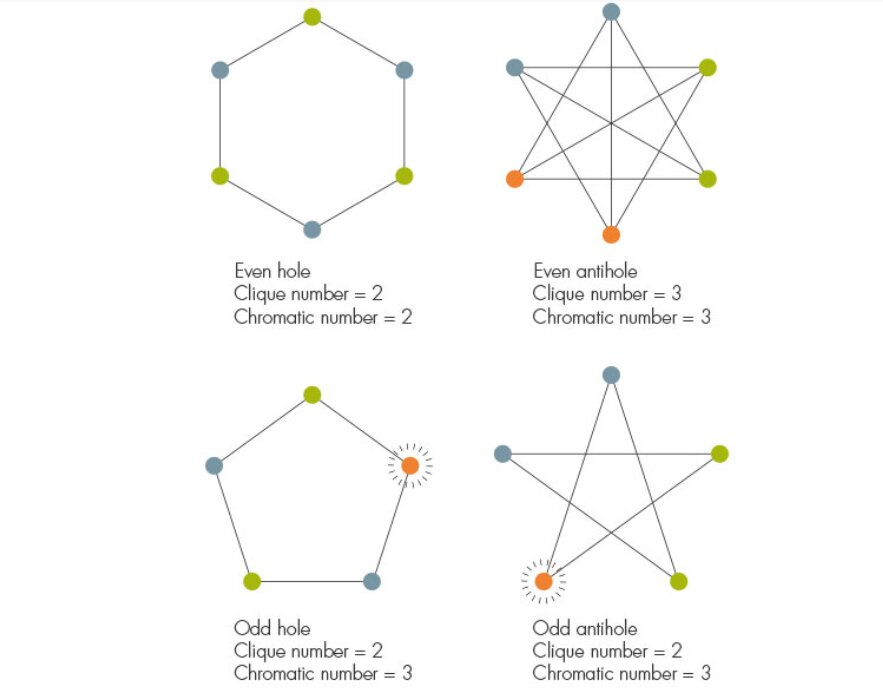
\includegraphics[scale=0.4]{images/graphproperty.jpg}
    \caption{Graph color and clique}
    \label{fig:example-image}\cite{quanta_image}
\end{figure*}
\section{TESTING CLIQUES AND INDEPENDENT SETS}                      
 We complete the proof of Theorem 1 in this section.The proof we describe applies to both the $\rho$-CLIQUE and the $\rho$-INDEPSET properties (by considering the complement of the
tested graph) but the latter fits in more naturally with the graph
container method, so in the rest of the section we discuss the
result entirely in terms of independent sets.
\subsection*{A. Container Shrinking Lemma}
\begin{lemma}[\textit{Container Shrinking Lemma}]
Let \( G = (V, E) \) be a graph on \( n \) vertices that is \(\epsilon\)-far from the \(\rho\)-INDEPSET property. Let \( I \) be an independent set in \( G \), and let \( t < |I| \) be an index for which the \( t \)-th container \( C_t \) of \( I \) has cardinality \( |C_t| \geq \rho n \). For any \(\alpha > 0\), if there exists a subset \( C \subseteq C_{t+1} \) of \( (\rho - \alpha)n \) vertices where \( G[C] \) contains at most \( \frac{\epsilon}{4} n^2 \) edges, then:
\begin{equation*}
|C_{t+1} \setminus C| \leq \left( 1 - \frac{\epsilon}{4 \rho \alpha} \right) |C_t \setminus C|
\end{equation*}
 
 We can now complete the proof of the claim that \( G[C_t \setminus C] \) contains at least \( \frac{\epsilon}{4 \rho \alpha} |C_t \setminus C|^2 \) edges.
Let \( R \) be chosen uniformly at random from all subsets of \( C_t \setminus C \) of size \( \alpha n \). Since \( G \) is \(\epsilon\)-far from having independent sets of size \( \rho n \), the induced subgraph \( G[R \cup C] \) contains at least \( \epsilon n^2 \) edges. By the lemma hypothesis, \( G[C] \) contains at most \( \frac{\epsilon}{4} n^2 \) edges. 
Finally, each edge connecting a vertex in \( C \) to one in \( C_t \setminus C \) is included in \( G[R \cup C] \) with probability \( \frac{|R|}{|C_t \setminus C|} \). So by the maximum degree of the vertices in \( C \) in the graph \( G[C_t] \), the expected number of edges between \( C \) and \( R \) is at most \( \frac{\epsilon}{4 \alpha} |R| n = \frac{\epsilon}{4} n^2 \). 
Therefore, the expected number of edges in \( G[R] \) is at least:
\begin{equation*}
\frac{\epsilon}{2} n^2 = \frac{\epsilon}{2 \alpha^2} |R|^2 \geq \frac{\epsilon}{\alpha^2} \binom{|R|}{2}
\end{equation*} 
\end{lemma}
\subsection*{B. . Proof of Graph Container Lemma I}
\subsubsection*{\textbf{Lemma 5}(Graph Container Lemma I)}
\begin{proof}
 Let $C$ denote the first container in the sequence $C_1, C_2, ...$ that contains at most $\frac{\epsilon}{4}n^2$ edges. The existence of C is guaranteed because $C_{|I|+1}$ is an independent set and has no edges. Define $\alpha$ such that $|C_{|I|+1}| = (p-\alpha)n$. The value of $\alpha$ is bounded by $\frac{\epsilon}{4p} \leq \alpha \leq p$, where the lower bound on $\alpha$ is due to the fact that G is $\epsilon$-far from the $\rho$-INDEPSET property.
Define $t^*$ to be the largest index for which $|C_t| \geq \rho n$. First observe that $t^* \leq |I|$ because otherwise $C_{t^*}$ is an independent set, which contradicts the fact that G is $\epsilon$-far from the $\rho$-INDEPSET property. Hence, by Lemma 7 applied to all values of t = 0, 1, 2, ..., $t^* - 1$,
$|C_{t^*} \setminus C| \leq (1 - \frac{\epsilon}{4\rho \alpha})^{t^*} n$
and since $|C_{t^*} \setminus C| \geq \alpha n$, we conclude that $t^* \leq \frac{4\rho \alpha}{\epsilon} \ln(1/\alpha) \leq \frac{4\rho \alpha}{\epsilon} \ln(2\rho/\epsilon)$.
\end{proof}
\subsection*{C.Proof of Theorem I}
\begin{lemma}[Chernoff’s Bound]
Let X be drawn from the
hypergeometric distribution $H(N, K, n)$ where $n$ elements are
drawn without replacement from a population of size N where
$K$ elements are marked and $X$ represents the number of
marked elements that were drawn. Then for any $\theta \geq E[X]$,
$Pr[X \geq \theta] \leq \exp \left( -\frac{(\theta - E[X])^2}{\theta + E[X]} \right)$.  
\end{lemma}
\subsubsection*{\textbf{Theorem 1}(Precise formulation).} The sample complexity of
the $\rho$-INDEPSET property is
\[\mathcal{S}_{\rho\cdot INDEPSET}(n,\epsilon)=O(\frac{\rho^{3}}{\epsilon^{2}}ln^{3}(\frac{1}{\epsilon}))\]
\begin{proof}
Let S be a random set of \(s=c\cdot\frac{\rho^{3}}{\epsilon^{2}}ln^{3}(\frac{1}{\epsilon})\) vertices
drawn uniformly at random from $V$ without replacement,
where $c$ is a large enough constant. Note that for clarity of
presentation, in the rest of the proof we ignore all integer
rounding issues as they do not affect the asymptotics of the
final result.
If $G$ contains a $\rho n$ independent set, then $S$ contains at least
$\rho s$ vertices from this independent set with probability at least
\(\frac{1}{2},\) since the number of such vertices follows a hypergeometric
distribution, and the median of this distribution is at least
$\rho s$  \cite{Neu70}\cite{KB80}.
In the remainder of the proof we upper bound the probability
that $S$ contains a $\rho s$-independent set when $G$ is $\epsilon$-far from
containing a $\rho n$-independent set. For the rest of the argument,let us call a container \(C_{t}\) small when its cardinality is bounded by 
$|C_t|\leq (\rho - t\cdot \frac{\epsilon}{8\rho \ln(2\rho/\epsilon)})n$  the expression (2) in the conclusion of Lemma 5. For the better understanding of the proof of the theorem .The related mathematical expressions with $i_1,i_2,i_3,....\in [s]$ :
\begin{align*}
E[X] &\leq \left(\rho - \frac{t\epsilon}{8\rho\ln\left(\frac{2\rho}{\epsilon}\right)}\right)(s-t) \nonumber \\
     &< \rho s - \frac{t\epsilon s}{8\rho\ln\left(\frac{2\rho}{\epsilon}\right)} \nonumber \\
     &\leq \rho s - t - \frac{t\epsilon s}{16\rho\ln\left(\frac{2\rho}{\epsilon}\right)},
\end{align*}


\begin{align*}
Pr[X \geq \rho s - t] \leq \exp \left( -\frac{(\rho s - t - E[X])^2}{\rho s - t + E[X]} \right) \\
\leq \exp \left( -\frac{t^2 \epsilon^2 s}{512 \rho^3 \ln^2(\frac{2 \rho}{\epsilon})} \right).
\end{align*}
Therefore, by applying a union bound over all values $t \leq \frac{8\rho^2 \ln(\frac{ 2\rho}{\epsilon})}{\epsilon}$
 and all possible choices of $t$ indices from $[s]$...
\begin{align*}
\sum_{t}\binom{s}{t} \exp ( -\frac{t^2 \epsilon^2 s}{512 \rho^3 \ln^2(\frac{2 \rho}{\epsilon})})\\
\leq \sum_{t}^{} \exp ( t \ln s - \frac{t^2 \epsilon^2 s}{512 \rho^3 \ln^2(\frac{2 \rho}{\epsilon})})< \frac{1}{3}
\end{align*}
\end{proof}
\section{TESTING K-COLORABILITY}
\subsubsection*{A. Proof of Graph Container Lemma II}
\textbf{Lemma 6}(Graph Container Lemma II).
Let G be $\epsilon$-far from
$k$-colorable, and let $I_1, \ldots, I_k$ be independent sets in G. Then,
there exists $t \leq \frac{4}{\epsilon}$ such that
\begin{align}
\left|\bigcup_{i=1}^{k} C_t(I_i)\right| \leq \left(1 - t \cdot \frac{\epsilon}{4 \ln(\frac{1}{\epsilon})}\right) n.
\tag{3}
\end{align}
Proof. Assume on the contrary that for all $t \leq 4/\epsilon$,
\begin{align}
\left|\bigcup_{i=1}^{k} C_t(I_i)\right| > \left(1 - t \cdot \frac{\epsilon}{4 \ln(\frac{1}{\epsilon})}\right) n.
\tag{4}
\end{align}

$\forall t = 1, \ldots, \frac{4}{\epsilon}$ ,Let  $A_t$  be the set of vertices that are contained in at least one container at the  $(t-1)$ -th step,but not contained in any container at step $t$  of the container procedure.
In other words, let 
\begin{align*}
A_t = \{v \in V: v \in \bigcup_{i \in [k]} C_{t-1}(I_i) \text{ and }\\
v \notin \bigcup_{i \in [k]} C_{t}(I_i) \}.
\end{align*}
The sum of the all edges in each of the sets $V_1,\ldots,V_k$ can be upper bounded by
\begin{equation}
\frac{\epsilon n^2}{4} + |A_1| \cdot n + \sum_{t=2}^{4/\epsilon} |A_t| \cdot \frac{n}{t-1}
\tag{5}
\end{equation}
Again the sum of the all edges in each of the sets $V_1,\ldots,V_k$ can be upper bounded by
\[
\frac{\epsilon n^2}{4} + \frac{\epsilon n^2}{4 \ln(1/\epsilon)} + \frac{\epsilon n^2}{4 \ln(1/\epsilon)} \sum_{t=2}^{4/\epsilon} \frac{1}{t-1} < \epsilon n^2,
\]
\subsection*{B. Proof of Theorem 2}
\textbf{Theorem 2} (Precise formulation). The sample complexity of
the $k$-COLORABLE property is
\[S_{k-COLORABLE}(n,\epsilon)=O\left(\frac{k}{\epsilon}\ln^{2}\left(\frac{1}{\epsilon}\right)\right).\]
\begin{proof}
$\forall t$,  there are at most  $\binom{s}{k} \leq s^{tk}$ ways to choose  $k$ sets of at most $t$ distinct indices as above. So by applying a union bound argument over all  $t \leq \frac{4}{\epsilon}$ and over all possible  $4k$ 
choices of indices, the probability that any set of at most$ \frac{4k}{\epsilon}$ vertices in  $S$ form the  $k$ fingerprints of a family of containers with a small union from which we sample all the remaining vertices is at most
\begin{align*}
\sum_{t=1}^{4/\epsilon} s^{tk} \left(1 - \frac{t \epsilon}{4 \ln(1/\epsilon)}\right)^{s-tk} \\
\leq \sum_{t=1}^{4/\epsilon} \exp \left( tk \ln(s) - \frac{t \epsilon s}{8 \ln(1/\epsilon)}\right) < \frac{1}{3}
\end{align*}   
\end{proof}
In conclusion, the container method provides a powerful framework for efficiently testing graph properties, particularly for determining whether a graph is far from containing large independent sets. By leveraging the shrinking of containers and probabilistic tools like Chernoff bounds, this method reduces the computational complexity involved in property testing. The approach ensures that only a small sample of vertices needs to be considered while maintaining high accuracy. Furthermore, the method's versatility makes it applicable to a range of other combinatorial optimization problems, offering a promising direction for future research in graph theory and algorithms.
\bibliographystyle{ieeetr}
\bibliography{ref}
\end{multicols}
\end{document}





